\subsection{Benchmarking instances}

This section shows how the instances have been generated. Possibly adding a very schematic pseudocode of our generation algorithm.\\

This section also explains the sets of instances that are prepared for the project:\\
\begin{itemize}
	\item small-medium set: used to compare the solving time of the ILP model versus the Metaheuristics models
	\item large set: used to test the Metaheuristics models parameters over a large set of instances in order the choose the best performing setup for each model.
\end{itemize} 

\subsubsection{The instance generator}

pseudocode\\
comments\\
how feasibility is assured\\
tests on how to increment solving time, including some graphs with the Best Integer and Best Bound evolution for different variations of the same instance\\
Conclusion on how to increase the "size" of the instance without computing the solving time of the ILP model.\\

The next figures show different executions of a small modification of a problem instance. In each figure, a parameter of the problem is modified to increase the time it takes to Cplex to solve the instance problem. This gives us an idea of what parameters increase the size of the problem instance.\\

\begin{center}
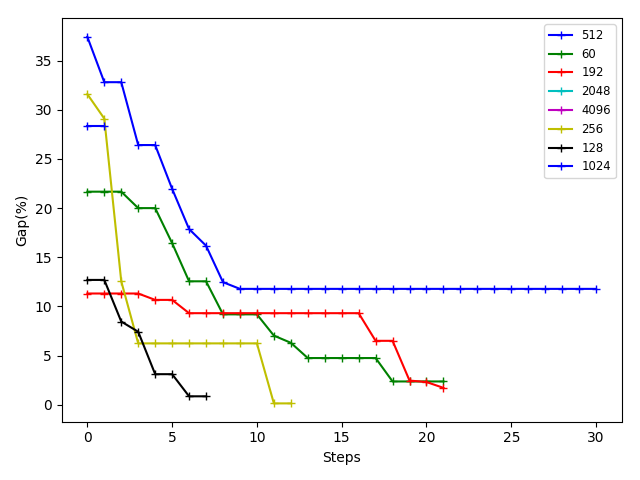
\includegraphics[width=0.5\textwidth]{./img/instances_nurses_ilp_evol.png}
\captionof{figure}{Evolution of Gap in similar problem instances with different number of nurses}
\end{center}

This chart shows that increasing the number of nurses increases the number of steps of the MILP problem to solve it.

\begin{center}
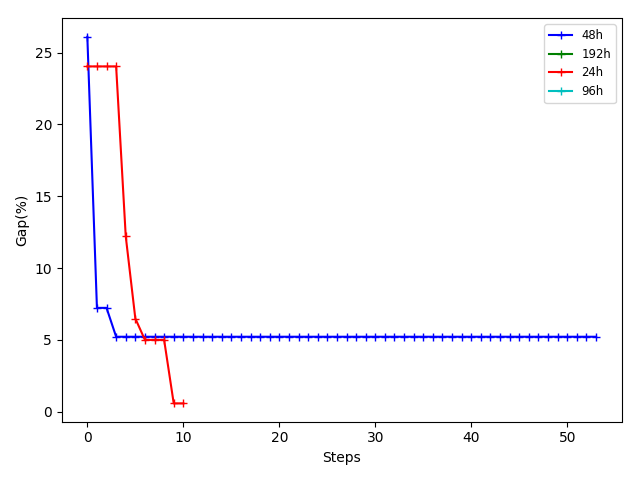
\includegraphics[width=0.5\textwidth]{./img/instances_hours_ilp_evol.png}\\[0.4cm] 
\captionof{figure}{Evolution of Gap in similar problem instances with different number of hours}
\end{center}

As we can observe in this chart, when the hours parameter increases, the number of steps to solve the MILP problem increases.


\begin{center}
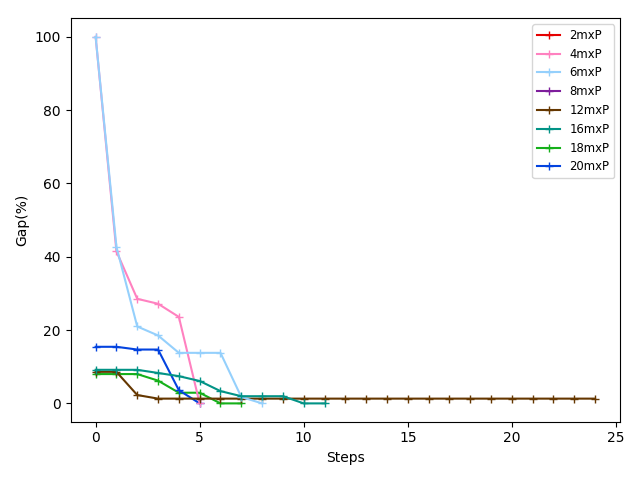
\includegraphics[width=0.5\textwidth]{./img/instances_maxpresence_ilp_evol.png}
\captionof{figure}{Evolution of Gap in similar problem instances with different values of maxPresence parameter}
\end{center}

This chart shows that decreasing the value of the maxPresence parameter increases the number of steps needed to solve the MILP problem.


\begin{center}
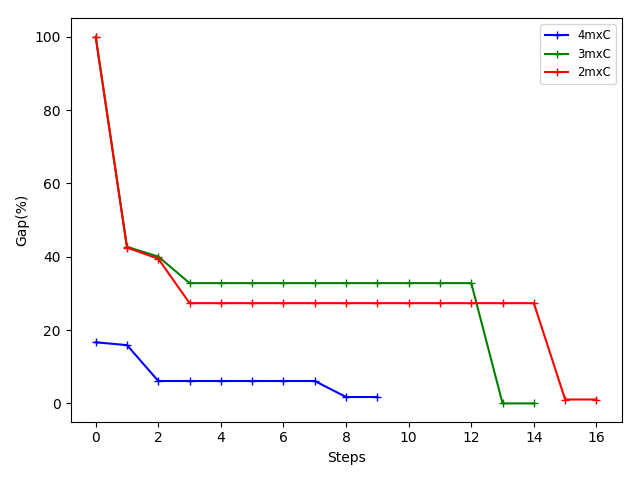
\includegraphics[width=0.5\textwidth]{./img/instances_maxconsec_ilp_evol.png}
\captionof{figure}{Evolution of Gap in similar problem instances with different values of maxConsec parameter}
\end{center}

The chart that shows the gap and the steps of the MILP problem for similar instances with different values of maxConsec parameter, allows us to conclude that decreasing the value of the maxConsec parameter increases the size of the problem.

\begin{center}
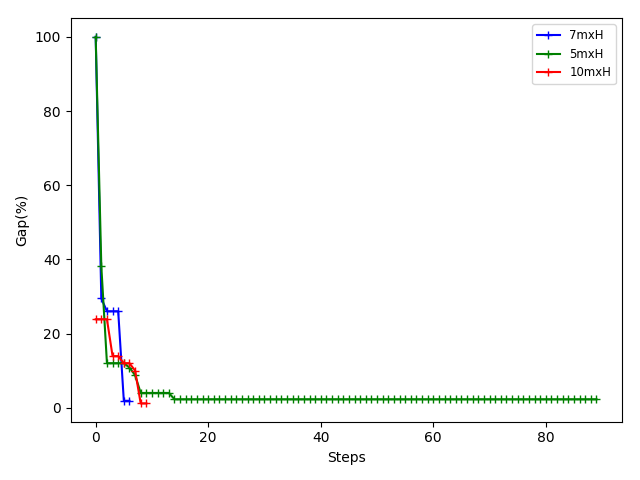
\includegraphics[width=0.5\textwidth]{./img/instances_maxhours_ilp_evol.png}
\captionof{figure}{Evolution of Gap in similar problem instances with different values of maxHours parameter}
\end{center} 

As we can see in this chart, the higher the maximum number of hours the nurses can work, the faster the MILP reduces the gap. In that case, reducing the number of maxHours parameter increases the size of the problem. 

\begin{center}
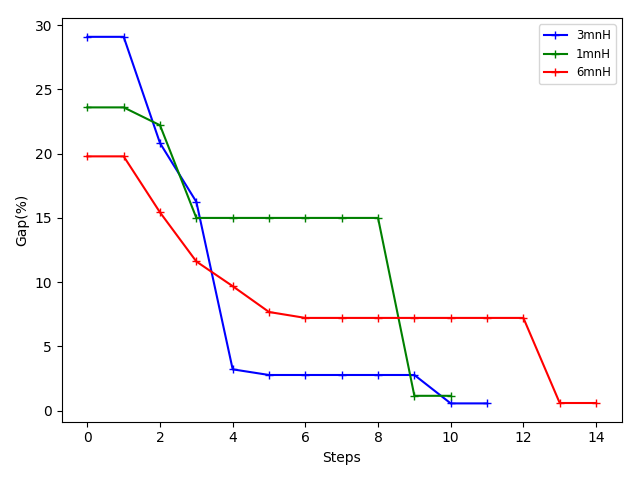
\includegraphics[width=0.5\textwidth]{./img/instances_minhours_ilp_evol.png}
\captionof{figure}{Evolution of Gap in similar problem instances with different values of minHours parameter}
\end{center}

We can observe in that last chart that if the minimum number of hours the nurses must work during a shift increases then the number of steps for the MILP to reduce the gap increases. So increasing the minHours parameters increases the size of the problem.


Those small observations allow us to conclude how the parameters of the MILP problem instance can be modified to increase its solving time. Thus we can increase the size of the problem by the following modifications:\\
\begin{itemize}
	\item increasing the number of nurses (nNurses)
	\item increasing the number of hours of the schedule (hours)
	\item decreasing the maximum presence hours (maxPresence)
	\item decreasing the maximum consecutive working hours (maxConsec)
	\item decreasing the maximum total working hours (maxHours)
	\item increasing the minimum total working hours (minHours)
\end{itemize}
The large set of problem instances will be generated using modifications of those parameters .


\subsubsection{Medium Set instances}

Composition of the set, number of instances and solving times.

\subsubsection{Large Set instances}

Composition of the set, number of instances, solving times or another measure of the size of the problem.


\pagebreak